\documentclass[a4paper, 12pt]{article}
\usepackage{graphicx}
\usepackage{listings, xcolor}
\usepackage{fancyvrb}


\definecolor{lightgray}{rgb}{.9,.9,.9}
\definecolor{darkgray}{rgb}{.4,.4,.4}
\definecolor{purple}{rgb}{0.65, 0.12, 0.82}
\lstdefinelanguage{JavaScript}{
	keywords={typeof, new, true, false, catch, function, return, null, catch, switch, var, if, in, while, do, else, case, break},
	keywordstyle=\color{blue}\bfseries,
	ndkeywords={class, export, boolean, throw, implements, import, this},
	ndkeywordstyle=\color{darkgray}\bfseries,
	identifierstyle=\color{black},
	sensitive=false,
	comment=[l]{//},
	morecomment=[s]{/*}{*/},
	commentstyle=\color{purple}\ttfamily,
	stringstyle=\color{red}\ttfamily,
	morestring=[b]',
	morestring=[b]"
}

\definecolor{verylightgray}{rgb}{.97,.97,.97}
\lstdefinelanguage{Solidity}{
	keywords=[1]{anonymous, assembly, assert, balance, break, call, callcode, case, catch, class, constant, continue, constructor, contract, debugger, default, delegatecall, delete, do, else, emit, event, experimental, export, external, false, finally, for, function, gas, if, implements, import, in, indexed, instanceof, interface, internal, is, length, library, log0, log1, log2, log3, log4, memory, modifier, new, payable, pragma, private, protected, public, pure, push, require, return, returns, revert, selfdestruct, send, solidity, storage, struct, suicide, super, switch, then, this, throw, transfer, true, try, typeof, using, value, view, while, with, addmod, ecrecover, keccak256, mulmod, ripemd160, sha256, sha3}, % generic keywords including crypto operations
	keywordstyle=[1]\color{blue}\bfseries,
	keywords=[2]{address, bool, byte, bytes, bytes1, bytes2, bytes3, bytes4, bytes5, bytes6, bytes7, bytes8, bytes9, bytes10, bytes11, bytes12, bytes13, bytes14, bytes15, bytes16, bytes17, bytes18, bytes19, bytes20, bytes21, bytes22, bytes23, bytes24, bytes25, bytes26, bytes27, bytes28, bytes29, bytes30, bytes31, bytes32, enum, int, int8, int16, int24, int32, int40, int48, int56, int64, int72, int80, int88, int96, int104, int112, int120, int128, int136, int144, int152, int160, int168, int176, int184, int192, int200, int208, int216, int224, int232, int240, int248, int256, mapping, string, uint, uint8, uint16, uint24, uint32, uint40, uint48, uint56, uint64, uint72, uint80, uint88, uint96, uint104, uint112, uint120, uint128, uint136, uint144, uint152, uint160, uint168, uint176, uint184, uint192, uint200, uint208, uint216, uint224, uint232, uint240, uint248, uint256, var, void, ether, finney, szabo, wei, days, hours, minutes, seconds, weeks, years},	% types; money and time units
	keywordstyle=[2]\color{teal}\bfseries,
	keywords=[3]{block, blockhash, coinbase, difficulty, gaslimit, number, timestamp, msg, data, gas, sender, sig, value, now, tx, gasprice, origin},	% environment variables
	keywordstyle=[3]\color{violet}\bfseries,
	identifierstyle=\color{black},
	sensitive=false,
	comment=[l]{//},
	morecomment=[s]{/*}{*/},
	commentstyle=\color{gray}\ttfamily,
	stringstyle=\color{red}\ttfamily,
	morestring=[b]',
	morestring=[b]"
}

\setlength\parindent{24pt}

\lstset{language=python,breaklines=true, frame=single}

\begin{document}
\begin{figure}
    \centering
    
\includegraphics[width=1\textwidth]{Logo}
\end{figure}

\title{Assignment 1 Report}
\author{Manwel Bugeja}
\date{\today}
\maketitle
  
\tableofcontents
\newpage

\section{Problem 1}

\section{Flow of the Contract}

\begin{figure}[h!]
	\centering
	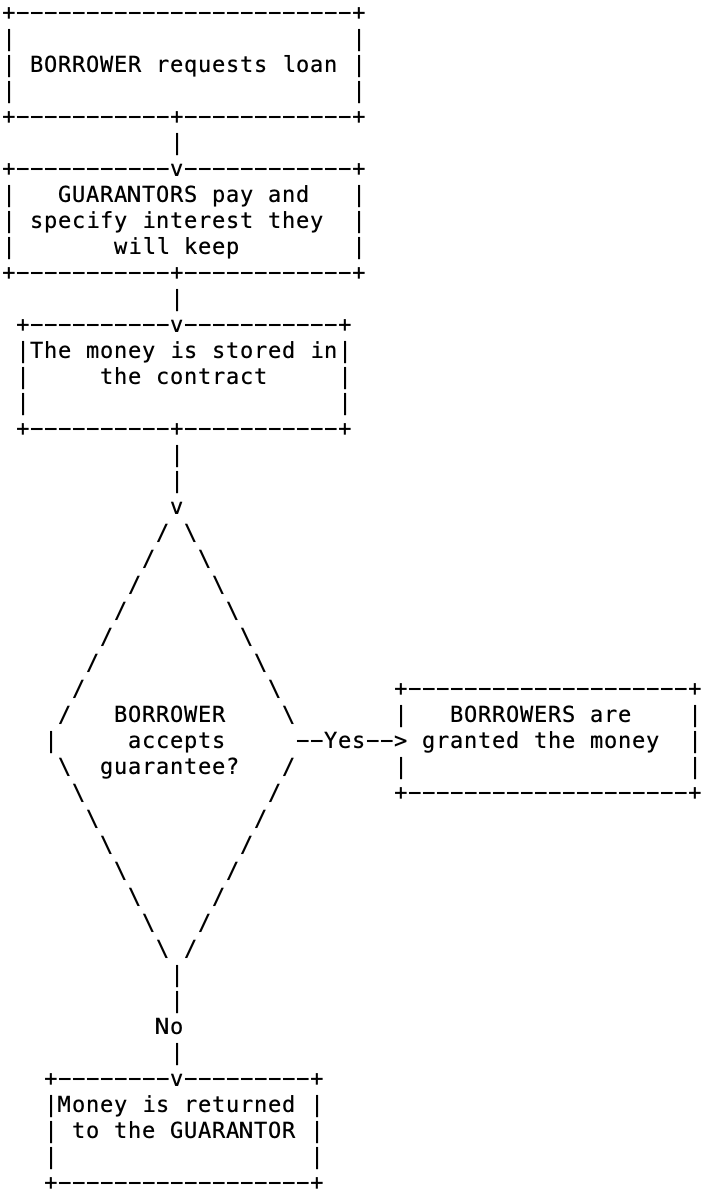
\includegraphics[width=\textwidth]{./Diagrams/problem1-flowchart}
	\caption{Submitting a Loan Request}
	\label{fig:flowchart1}
	% reference with \ref{fig:mesh1}
\end{figure}


\begin{figure}[h!]
	\centering
	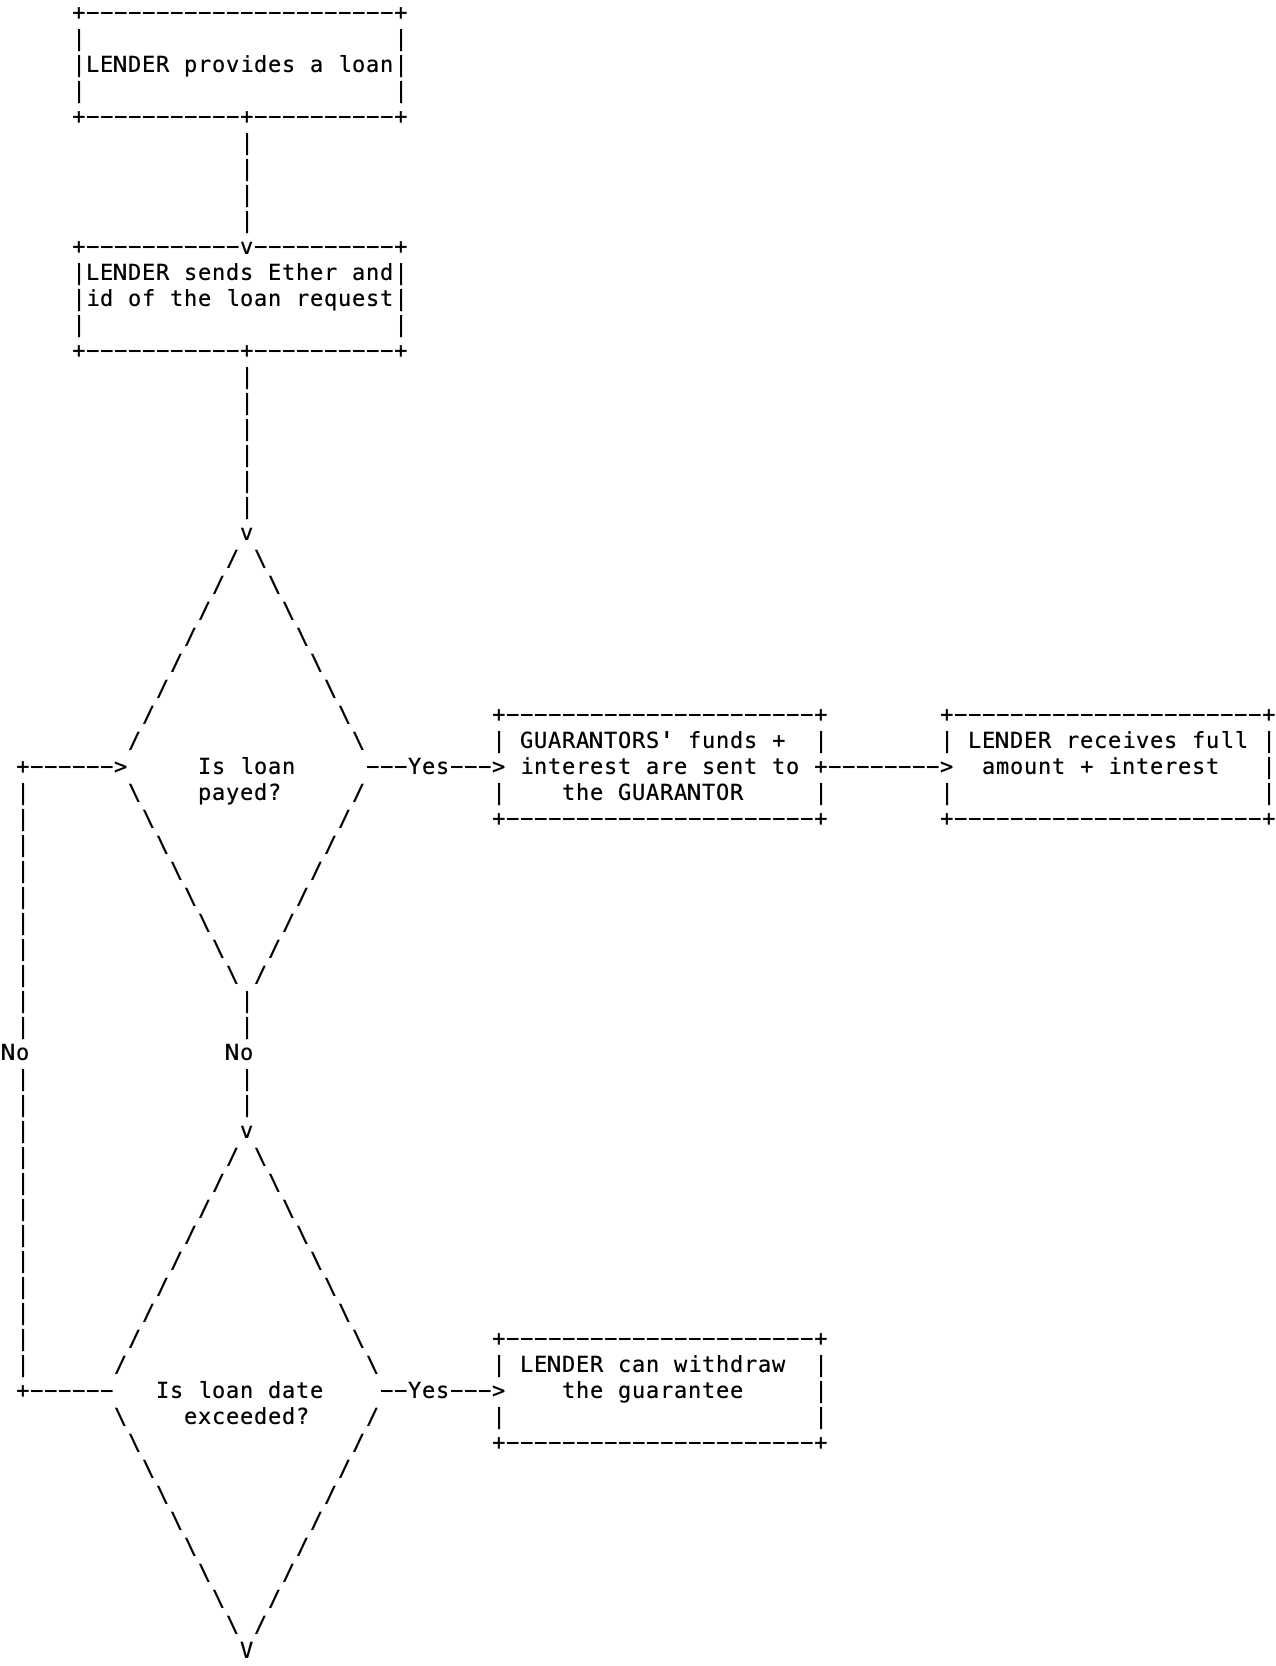
\includegraphics[width=\textwidth]{./Diagrams/problem1-flowchart2}
	\caption{Submitting a Loan}
	\label{fig:flowchart2}
	% reference with \ref{fig:mesh1}
\end{figure}

The flow of the process is shown via a flowchart in figures \ref{fig:flowchart1} and \ref{fig:flowchart2}.


\subsection{Structures}

The most fundamental part of the contract is a structure for loan requests, \textit{LoanRequest}. 
This can be seen in listing \ref{lst:LoanRequestStruct}. This structure contains the information required regarding the three persons included in the deal, i.e. the borrower, the guarantor and the loaner.

\begin{lstlisting}[caption={Loan Request Structure}\label{lst:LoanRequestStruct}, basicstyle=\ttfamily, frame=single, language=Solidity]
struct LoanRequest{
	uint    creationDate;       
	
	address payable borrower;
	uint    amount;             // Amount to be borrowed
	uint    expiryTime;         // Max time (in seconds) the loan will be paid back
	uint    interestPaid;       // Amount (in wei) paid on loan payback
	
	address payable guarantor; 
	uint    guarantorInterest;  // Amount (in wei) taken from interest by the guarantor
	
	address payable loaner;     
	State   state;            
}
\end{lstlisting}

The last field of the loan request structure is an enumeration called \textit{State}, which can be seen in listing \ref{lst:StateEnum}. This enumeration contains the information about what state the loan request resides in. The states are explained in table \ref{tab:StateEnum}.


	
\begin{lstlisting}[caption={Loan Request Structure}\label{lst:StateEnum}, basicstyle=\ttfamily, frame=single, language=Solidity]
enum State {
	REQUESTED,
	PENDING,
	GUARANTEED,
	LOANED,
	PAID,
	TERMINATED
}
\end{lstlisting}

\begin{center}
	\resizebox{\textwidth}{!}{\begin{tabular}{ |c| c| }
			\hline
			\textbf{State} & \textbf{Description} \\ 
			\hline
			REQUESTED    & The borrower submitted a request  \\  
			\hline
			PENDING         &The guarantor submitted a guarantee and is waiting for approval \\
			\hline
			GUARANTEED & The guarantee has been accepted by the borrower\\
			\hline
			LOANED          & The loaner has loaned the money\\
			\hline
			PAID                & The borrower paid the loaner back before the loan expired\\
			\hline
			TERMINATED   & The loan expired and the loaner took the guarantee\\
			\hline
	\end{tabular}}
	\label{tab:StateEnum}
\end{center}

These loan requests are all kept in a dynamic array, \textit{LoanRequests[]}. Elements are added to this array from the functions. However, elements are never removed. This allows the system to keep a log of all requests ever made.

\subsection{Functions}

Functions in the contract are split into four sections, these being: general purpose, borrower, guarantor and loaner functions.
\\
General purpose functions are mostly used to get information about the loan requests. This means that most of them include the \textit{view} keyword.
\\
Functions that act on a created loan request take the index as a parameter. Furthermore, the functions have the following flow: checks, followed by code that transfer balance, followed by updating the loan request states. The reason for this is explain in the section about security. 

\subsection{Testing and Error checking}
The functions that are to be executed by users of a specific role (borrower, guarantor or loaner) have checks at the start to ensure validity. These checks are done using the \textit{require} function so useful messages are outputted. 
\\
For example, referring to listing \ref{lst:GuaranteeSubmissionChecks} when submitting a guarantee the check done are: checking that the request is in state \textit{REQUESTED}; checking that the amount of balance given by the guarantor is more that the amount requested by the borrower; and finally, checking that the interest to be taken by the guarantor is less than the interest the borrower will provide.

\begin{lstlisting}[caption={Loan Request Structure}\label{lst:GuaranteeSubmissionChecks}, basicstyle=\ttfamily, frame=single, language=Solidity]
require(loanRequests[index].state == State.REQUESTED,   "Loan in invalid state");   
require(msg.value >= loanRequests[index].amount,        "Insufficient balance given");
require(loanRequests[index].interestPaid > interest,    "Guarantor interest must be less than Borrower interest");
\end{lstlisting}

Testing the functions in task 1 was done manually via the Remix IDE. The functionality was tested to be working as should with the provided interface and that in the case of misuse, a useful error message was printed. The feature to use multiple account was also used.
\\
For example if a guarantor wanted to try and accept his own guarantee, the checks would not pass and the error message "Caller is not Borrower" would provided as shown in figure \ref{fig:error}.

\begin{figure}[h!]
	\centering
	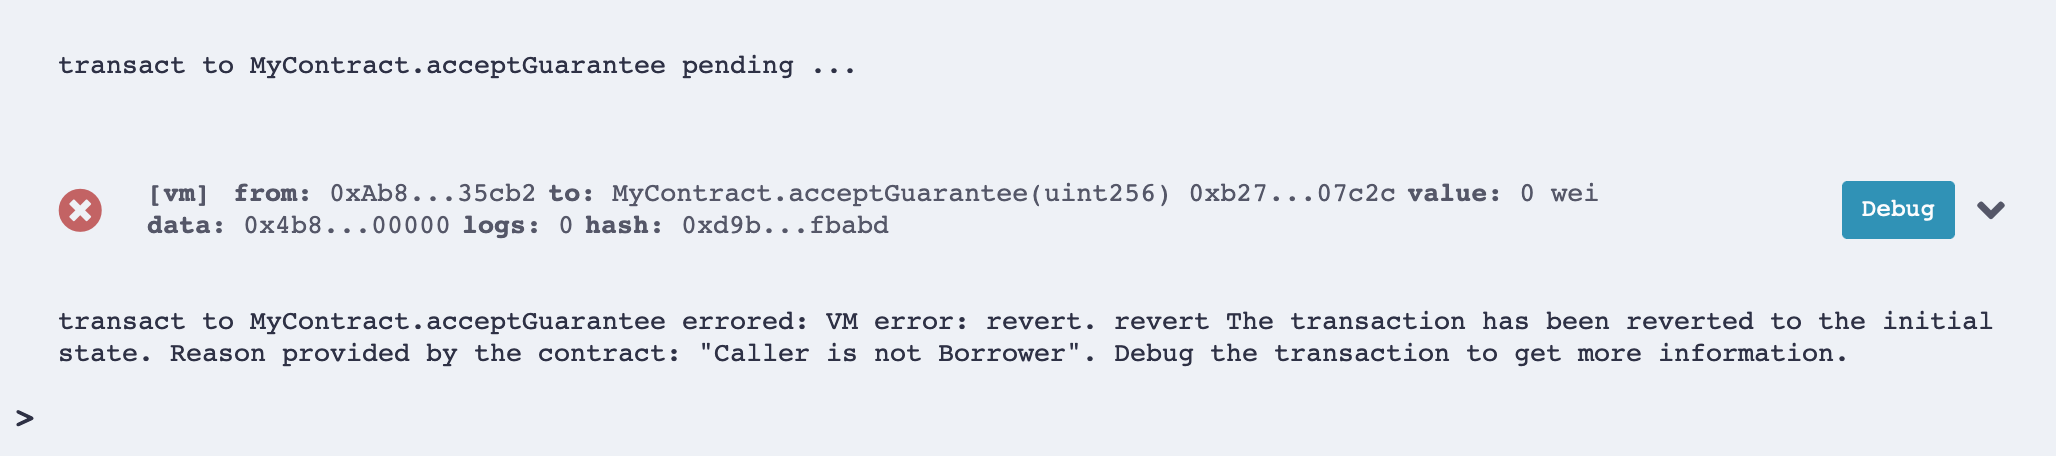
\includegraphics[width=\textwidth]{./Images/error}
	\caption{Guarantor Accepting his Own Guarantee}
	\label{fig:error}
	% reference with \ref{fig:mesh1}
\end{figure}


\section{Problem 2}
\section{Problem 3}
JavaScript tests were written using the \textit{async} method. Tests were conducted for all functions and different accounts were used. Listing \ref{lst:TestMultipleAccounts} show how multiple accounts were used to simulate multiple people. 

\begin{lstlisting}[caption={Multiple accounts in testing}\label{lst:TestMultipleAccounts}, basicstyle=\ttfamily, frame=single, language=JavaScript]
contract('MyContract', accounts => {
	const borrower = accounts[0];
	const guarantor = accounts[1];
	const loaner = accounts[2];
	...
}
\end{lstlisting}

Tests that were made manually om the remix IDE were replicated with these types of tests. Considering the same example as before, where a guarantor might try to accept his own guarantee, the test is shown in listing \ref{lst:TestMisuse}.

\begin{lstlisting}[caption={Guarantor accepting his own guarantee test}\label{lst:TestMisuse}, basicstyle=\ttfamily, frame=single, language=JavaScript]

it('testing a guarantor accepting his own guarantee', async() => {
	const contract = await MyContract.deployed();
	await contract.submitLoanRequest(200, 100000, 20, {from: borrower});
	await contract.guaranteeLoan(3, 10, {value: 500, from: guarantor});
	
	try {
		await contract.acceptGuarantee(3, {from: guarantor});
	} catch (error) {
		assert.equal(error.reason, "Caller is not Borrower")
	}
});

\end{lstlisting}

\begin{lstlisting}[caption={Borrower submitting a load request}, basicstyle=\ttfamily, frame=single, language=JavaScript]
  
it('testing submitting a loan request', async () => {
	const contract = await MyContract.deployed();
	await contract.submitLoanRequest(200, 1614786990, 20, { value: 0, account: borrower });
	await contract.submitLoanRequest(300, 1614786990, 18, { value: 0, account: borrower });
	let ret = await contract.getLoanRequestCount.call();
	assert(ret.toNumber() == 2);
});

\end{lstlisting}

Tests were conducted for all functions that change the state of the contract i.e. all of them except the getters.
There are several tests for each function because there are several invalid ways to use a function and only one good/valid way. The tests test for all invalid uses hence triggering all \textit{require} calls. This enables the system to be more robust.

\section{Problem 4}
First off, the file \textit{truffle-config.js} was edited to add metamask and infura. The rinkeby live test network was used. Then npx was installed and a react app was created. 
\\

Then \textit{App.js} was edited to display the required fields for contract interaction. Listing \ref{lst:WebSubmit} show the back end of submitting a loan request. While figures \ref{fig:webSubmit} and \ref{fig:webConfirm} show submitting and confirming a loan request from the web ui. After that, when the transaction is successfully updated, the count above the form is also updated.

\begin{lstlisting}[caption={Submitteing a borrow request from web}\label{lst:WebSubmit}, basicstyle=\ttfamily, frame=single, language=JavaScript]
	
	  submitLoanRequest = async (event) => {
		event.preventDefault();
		var accounts = await web3.eth.getAccounts();
		var myContract = myContract = new web3.eth.Contract(abi, contractAddress);
		await myContract.methods.submitLoanRequest(this.state.loanRequestAmount, this.state.loanRequestTime, this.state.loanRequestInterest).send({
			from: accounts[this.state.accountNum]
		});
		this.updateState();
	}
	
\end{lstlisting}

\begin{figure}[h!]
	\centering
	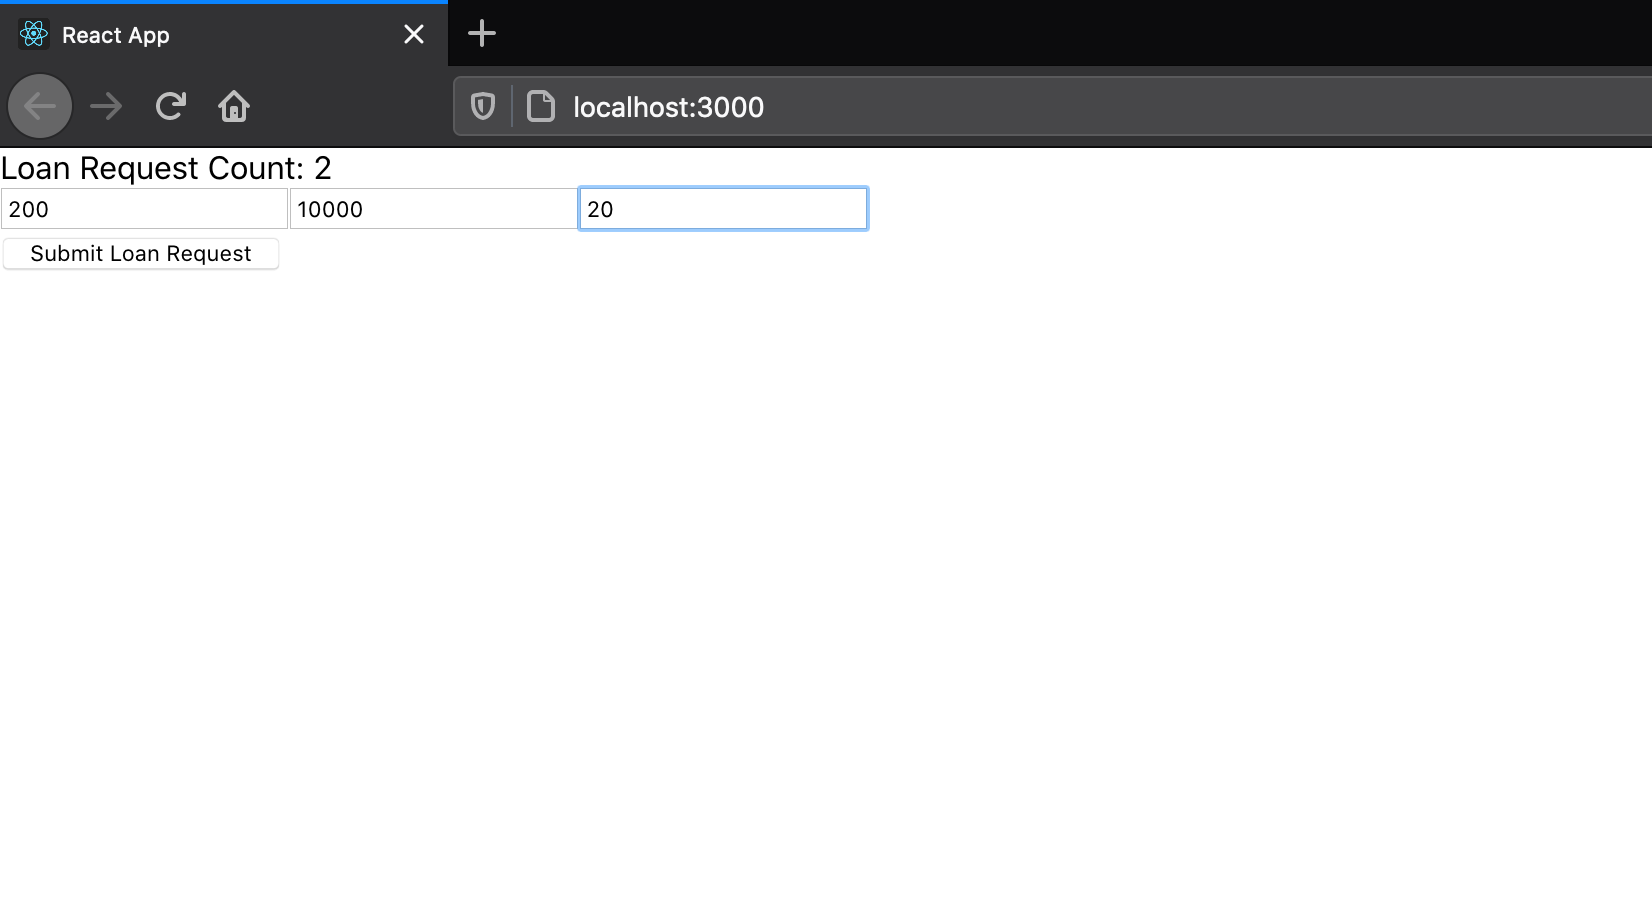
\includegraphics[width=\textwidth]{./Images/webSubmit}
	\caption{Because question 5 is the report itself}
	\label{fig:webSubmit}
	% reference with \ref{fig:mesh1}
\end{figure}

\begin{figure}[h!]
	\centering
	\includegraphics[width=\textwidth]{./Images/Confirm}
	\caption{Because question 5 is the report itself}
	\label{fig:webConfirm}
	% reference with \ref{fig:mesh1}
\end{figure}

\section{Problem 5}
For this problem please refer to figure \ref{fig:obi}.

\begin{figure}[h!]
	\centering
	
\includegraphics[width=\textwidth]{./Images/obi}
	\caption{Because question 5 is the report itself}
	\label{fig:obi}
	% reference with \ref{fig:mesh1}
\end{figure}

%\bibliographystyle{abbrv}
 %\bibliography{references}

\end{document}
